\documentclass[aspectratio=169,11pt,t]{beamer}

% ============================================================
% Theme and typography
% ============================================================

\usetheme{Madrid}
\usecolortheme{default}
\usefonttheme{professionalfonts}

\setbeamertemplate{navigation symbols}{}
\setbeamertemplate{headline}{}

\setbeamertemplate{footline}{%
  \leavevmode\hbox{%
  \begin{beamercolorbox}[wd=.82\paperwidth,ht=2.5ex,dp=1.0ex,leftskip=.8em]{author in head/foot}
    CSCI 6461 --- Computer Systems Architecture
  \end{beamercolorbox}%
  \begin{beamercolorbox}[wd=.18\paperwidth,ht=2.5ex,dp=1.0ex,rightskip=.8em]{date in head/foot}
    \hfill\insertframenumber/\inserttotalframenumber
  \end{beamercolorbox}}
}

\setbeamersize{
  text margin left=0.65cm,
  text margin right=0.65cm
}

\setbeamerfont{frametitle}{size=\Large, series=\bfseries}
\setbeamerfont{block title}{size=\normalsize, series=\bfseries}
\setbeamertemplate{blocks}[rounded][shadow=false]

% Block vertical padding adjustments
\addtobeamertemplate{block begin}{\vspace{0.1em}}{\vspace{0.1em}}
\addtobeamertemplate{block end}{}{\vspace{0.2em}}

% Base list item separation
\setbeamertemplate{itemize/enumerate body begin}{\setlength{\itemsep}{4pt}}
\setbeamertemplate{itemize/enumerate subbody begin}{\setlength{\itemsep}{2pt}}

% ============================================================
% Packages
% ============================================================

\usepackage[T1]{fontenc}
\usepackage{lmodern}
\IfFileExists{sourcecodepro.sty}{\usepackage[scale=0.92]{sourcecodepro}}{\usepackage{courier}}
\usepackage{amsmath}
\usepackage{booktabs}
\usepackage{array}
\usepackage{tikz}

\usetikzlibrary{
  arrows.meta,
  positioning,
  shapes.geometric,
  calc,
  decorations.pathreplacing
}

% ============================================================
% Colors
% ============================================================

\definecolor{navy}{RGB}{24,43,68}
\definecolor{deepblue}{RGB}{45,88,130}
\definecolor{lightblue}{RGB}{235,242,250}
\definecolor{softgray}{RGB}{245,247,250}
\definecolor{darkgray}{RGB}{25,28,32}
\definecolor{gold}{RGB}{200,145,35}

\setbeamercolor{palette primary}{bg=navy,fg=white}
\setbeamercolor{palette secondary}{bg=deepblue,fg=white}
\setbeamercolor{frametitle}{bg=navy,fg=white}
\setbeamercolor{title}{fg=white}
\setbeamercolor{subtitle}{fg=white}
\setbeamercolor{author}{fg=white}
\setbeamercolor{date}{fg=white}
\setbeamercolor{titlelike}{fg=white}
\setbeamercolor{block title}{bg=deepblue,fg=white}
\setbeamercolor{block body}{bg=lightblue,fg=darkgray}
\setbeamercolor{normal text}{fg=darkgray,bg=white}

% ============================================================
% Formatting shortcuts
% ============================================================

\setlength{\parskip}{0pt}

\newcommand{\key}[1]{\textbf{#1}}
\newcommand{\bits}[1]{\texttt{#1}}
\newcommand{\hex}[1]{\texttt{0x#1}}
\newcommand{\code}[1]{\texttt{#1}}

% Section divider macro
\newcommand{\sectiondivider}[2]{%
\begin{frame}[plain]
\begin{tikzpicture}[remember picture,overlay]
\fill[navy] (current page.south west) rectangle (current page.north east);
\fill[gold] (current page.south west) rectangle ([yshift=.15cm]current page.south east);
\end{tikzpicture}
\vspace{1.5cm}
\begin{minipage}{0.85\textwidth}
{\color{gold}\large\bfseries #1\par}
\vspace{0.3cm}
{\color{white}\fontsize{22}{26}\selectfont\bfseries #2\par}
\end{minipage}
\end{frame}
}

% ============================================================
% Metadata
% ============================================================

\title[Topic 6]{
  Subroutines, Calling Conventions, \& the Stack
}

\subtitle{
  Function linkage, register preservation rules, stack frame management,\\
  and AAPCS64 architectural compliance
}

\author{
  Computer Systems Architecture
}

\date{}

% ============================================================
% Document
% ============================================================

\begin{document}

% ============================================================
% Slide 1: Title Slide
% ============================================================

\begin{frame}[plain]
\begin{tikzpicture}[remember picture,overlay]
\fill[navy] (current page.south west) rectangle (current page.north east);
\fill[gold] (current page.south west) rectangle ([yshift=.15cm]current page.south east);
\end{tikzpicture}

\vspace{0.8cm}
\begin{minipage}{0.88\textwidth}
{\color{gold}\normalsize\bfseries CSCI 6461 \;|\; TOPIC 6\par}
\vspace{0.25cm}
{\color{white}\fontsize{24}{28}\selectfont\bfseries
 Subroutines, Calling Conventions,\\[0.08cm]
 \& the Stack
\par}
\vspace{0.35cm}
{\color{white!80}\large
 Function linkage, register preservation rules, stack frame management,\\
 and AAPCS64 architectural compliance
\par}
\end{minipage}

\vfill
{\color{white}\normalsize Dr. J. Burns\par}
{\color{white!70}\small Computer Systems Architecture --- AArch64 Reference Platform\par}
\vspace{0.35cm}
\end{frame}

% ============================================================
% Slide 2: Module Overview
% ============================================================



% ============================================================
% Section 1 Divider
% ============================================================

\sectiondivider{PART 1}{Subroutine Linkage \& Control Flow}

% ============================================================
% Slide 3
% ============================================================

\begin{frame}{High-Level Function Execution Model}
\large
\begin{itemize}\setlength{\itemsep}{7pt}
  \item \key{Subroutines} provide modular abstraction, reusability, and clean software architecture.
  \item To execute a function call, the CPU must satisfy five core requirements:
  \begin{enumerate}\setlength{\itemsep}{3pt}
    \item \key{Pass Arguments:} Transfer input parameters to the function.
    \item \key{Transfer Control:} Jump to the function's entry point address.
    \item \key{Isolate Local State:} Provide memory space for function local variables.
    \item \key{Return Value:} Pass computed results back to the caller.
    \item \key{Resume Execution:} Return seamlessly to the instruction following the call.
  \end{enumerate}
\end{itemize}
\end{frame}

% ============================================================
% Slide 4
% ============================================================

\begin{frame}{The Link Register (\texttt{x30}) and Branch-with-Link (\texttt{bl})}

\begin{itemize}\setlength{\itemsep}{6pt}
  \item Invoking a function requires remembering where to return when it completes.
  \item \key{Branch with Link (\code{bl label}):} Atomically performs two operations:
  \begin{enumerate}\setlength{\itemsep}{2pt}
    \item Saves return address ($\text{PC} + 4$) into the \key{Link Register (\bits{x30} / \bits{lr})}.
    \item Branches to target function: $\text{PC} \leftarrow \text{label}$.
  \end{enumerate}
\end{itemize}

\vspace{0.2cm}
\centering
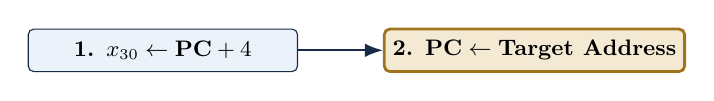
\begin{tikzpicture}[scale=0.9, every node/.style={transform shape}]
  \node[draw=navy, fill=lightblue, rounded corners=2pt, minimum width=3.8cm, minimum height=0.6cm, font=\small\bfseries] (save) {1. $x_{30} \leftarrow \text{PC} + 4$};
  \node[draw=gold!80!black, fill=gold!20, line width=1pt, rounded corners=2pt, right=1.2cm of save, minimum width=3.2cm, minimum height=0.6cm, font=\small\bfseries] (jump) {2. $\text{PC} \leftarrow \text{Target Address}$};
  \draw[-{Latex}, thick, navy] (save) -- (jump);
\end{tikzpicture}

\vspace{0.3cm}
\begin{block}{PC-Relative Calling Range}
The \code{bl} instruction encodes a signed 26-bit immediate offset, allowing direct function calls within a $\pm 128\text{ MB}$ window of the current instruction.
\end{block}
\end{frame}

% ============================================================
% Slide 5
% ============================================================

\begin{frame}{Subroutine Return Mechanics (\texttt{ret})}
\large
\begin{itemize}\setlength{\itemsep}{6pt}
  \item \key{Return from Subroutine (\code{ret}):} Branches to the address held in a register. With no explicit operand, \code{ret} uses the link register \bits{x30}:
  $$\text{PC} \leftarrow x_{30}$$
  \item A normal \code{bl} / \code{ret} pair therefore resumes at the instruction following the original call.
\end{itemize}

\vspace{0.15cm}
\begin{block}{Example: Minimal Leaf Return Sequence}
\small
\begin{tabular}{ll}
\code{caller\_func:} & \\
\quad \code{bl  helper\_func}  & \text{\scriptsize // x30 = return address; branch to helper} \\
\quad \code{mov x1, x0}        & \text{\scriptsize // resumes here after ret} \\
\code{helper\_func:} & \\
\quad \code{add x0, x0, \#1}  & \text{\scriptsize // compute result} \\
\quad \code{ret}               & \text{\scriptsize // default target register is x30} \\
\end{tabular}
\end{block}
\end{frame}

% ============================================================
% Slide 6
% ============================================================

\begin{frame}{Leaf vs.\ Non-Leaf Functions}
\begin{columns}[T,onlytextwidth]
\begin{column}{0.48\textwidth}
\begin{block}{Leaf Functions}
\begin{itemize}\setlength{\itemsep}{3pt}
  \item Call \key{no other functions}.
  \item \bits{x30} is not overwritten by a nested \code{bl}.
  \item May still use stack space for locals or spills, but need not save \bits{x30} solely for linkage.
\end{itemize}
\end{block}
\end{column}
\begin{column}{0.48\textwidth}
\begin{block}{Non-Leaf Functions}
\begin{itemize}\setlength{\itemsep}{3pt}
  \item Call one or more \key{nested subroutines}.
  \item A nested \code{bl} overwrites \bits{x30} with the nested return address.
  \item Preserve the incoming return address before that happens if it will be needed later.
\end{itemize}
\end{block}
\end{column}
\end{columns}
\vspace{0.2cm}
\begin{block}{The Non-Leaf Rule}
If a function makes another call and must later return to its own caller, its incoming return address must be preserved before \bits{x30} is overwritten.
\end{block}
\end{frame}

% ============================================================
% Slide 7
% ============================================================

\begin{frame}{Indirect Subroutine Calls (\texttt{blr})}
\large
\begin{itemize}\setlength{\itemsep}{6pt}
  \item When the target function address is determined dynamically at runtime, use \key{Branch with Link to Register (\code{blr xn})}.
  \item Saves return address ($\text{PC} + 4$) into \bits{x30} and jumps to address held in register \bits{xn}.
\end{itemize}

\vspace{0.2cm}
\begin{block}{Primary Applications}
\begin{itemize}\setlength{\itemsep}{3pt}
  \item \key{C Function Pointers:} \code{void (*func\_ptr)(int) = my\_callback;}
  \item \key{Virtual Method Tables (vtables):} C++ polymorphism and object dispatch.
  \item \key{Shared Library Veneers:} Dynamic linking and Symbol Jump Tables.
\end{itemize}
\end{block}

\vspace{0.2cm}
\small
\code{ldr x2, [x0, \#8]} \quad \text{\scriptsize // Load function pointer from vtable} \\
\code{blr x2}             \quad \text{\scriptsize // Call function indirectly via register x2}
\end{frame}

% ============================================================
% Slide 8
% ============================================================

\begin{frame}{Subroutine Call Execution Trace}
\centering
\vspace{0.1cm}
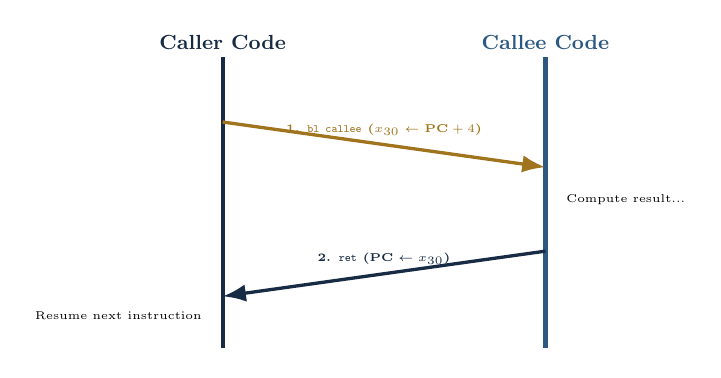
\begin{tikzpicture}[scale=0.82, every node/.style={transform shape}]
  \draw[navy, line width=1.5pt] (0,0) -- (0,4.5);
  \node[anchor=south, font=\small\bfseries, navy] at (0,4.5) {Caller Code};
  \draw[deepblue, line width=1.5pt] (5,0) -- (5,4.5);
  \node[anchor=south, font=\small\bfseries, deepblue] at (5,4.5) {Callee Code};
  \draw[-{Latex}, gold!80!black, line width=1.2pt] (0,3.5) -- (5,2.8)
    node[midway, above, font=\tiny\bfseries] {1. \code{bl callee} ($x_{30} \leftarrow \text{PC}+4$)};
  \node[anchor=west, font=\tiny] at (5.2,2.3) {Compute result...};
  \draw[-{Latex}, navy, line width=1.2pt] (5,1.5) -- (0,0.8)
    node[midway, above, font=\tiny\bfseries] {2. \code{ret} ($\text{PC} \leftarrow x_{30}$)};
  \node[anchor=east, font=\tiny] at (-0.2,0.5) {Resume next instruction};
\end{tikzpicture}
\vspace{0.2cm}
\normalsize
Control transfers from caller to callee and back using \bits{x30} to hold the return address.
\end{frame}

% ============================================================
% Section 2 Divider
% ============================================================

\sectiondivider{PART 2}{Procedure Call Standard \& Register Roles}

% ============================================================
% Slide 9
% ============================================================

\begin{frame}{Purpose of Procedure Call Standards (AAPCS64)}
\large
\begin{itemize}\setlength{\itemsep}{6pt}
  \item \key{AAPCS64:} Procedure Call Standard for the ARM 64-bit Architecture.
  \item Defines the calling-convention contract between independently compiled caller and callee functions.
  \item \key{Why the ABI Contract Matters}
  \begin{itemize}\setlength{\itemsep}{3pt}
    \item Allows assembly code to call C library functions such as \code{printf} and \code{malloc}.
    \item Enables code generated by different compilers to interoperate.
    \item Defines parameter passing, return values, stack use, and register-preservation rules.
  \end{itemize}
\end{itemize}
\end{frame}

% ============================================================
% Slide 10
% ============================================================

\begin{frame}{Parameter Passing Registers (\texttt{x0}--\texttt{x7})}
\large
\begin{itemize}\setlength{\itemsep}{5pt}
  \item Up to \key{eight 64-bit scalar integer or pointer arguments} can be passed in \bits{x0} through \bits{x7}, subject to AAPCS64 argument-classification rules.
\end{itemize}
\vspace{0.1cm}
\begin{center}
\small
\setlength{\tabcolsep}{6pt}
\begin{tabular}{cll}
\toprule
\textbf{Parameter Index} & \textbf{Register} & \textbf{C Language Example} \\
\midrule
1st Argument & \bits{x0} (\bits{w0}) & \code{int64\_t a} \\
2nd Argument & \bits{x1} (\bits{w1}) & \code{char *str} \\
3rd Argument & \bits{x2} (\bits{w2}) & \code{size\_t length} \\
4th--8th Arguments & \bits{x3}--\bits{x7} & Additional scalar arguments \\
\bottomrule
\end{tabular}
\end{center}
\vspace{0.15cm}
\begin{block}{Additional Arguments}
Arguments not assigned to registers are placed in the stack argument area according to AAPCS64 layout and classification rules.
\end{block}
\end{frame}

% ============================================================
% Slide 11
% ============================================================

\begin{frame}{Return Value Registers}
\begin{itemize}\setlength{\itemsep}{5pt}
  \item Many scalar return values are returned directly in registers.
\end{itemize}
\vspace{0.1cm}
\begin{center}
\footnotesize
\renewcommand{\arraystretch}{1.15}
\begin{tabular}{>{\raggedright\arraybackslash}p{0.28\textwidth} >{\raggedright\arraybackslash}p{0.18\textwidth} >{\raggedright\arraybackslash}p{0.40\textwidth}}
\toprule
\textbf{Return Data} & \textbf{Register(s)} & \textbf{Typical Rule} \\
\midrule
32-bit scalar integer / Boolean & \bits{w0} & Result returned in the lower 32-bit view. \\
64-bit scalar integer / pointer & \bits{x0} & Result returned in register 0. \\
Suitable integer-like aggregate up to 16 bytes & \bits{x0}, \bits{x1} & May use two general-purpose result registers. \\
Larger or non-register aggregate & indirect via \bits{x8} & Caller supplies an indirect result location when required. \\
\bottomrule
\end{tabular}
\end{center}
\vspace{0.15cm}
\begin{block}{Scope Note}
Floating-point and SIMD return rules use the SIMD/FP register file and are outside this lecture's focus.
\end{block}
\end{frame}

% ============================================================
% Slide 12
% ============================================================

\begin{frame}{Caller-Saved Registers (\texttt{x0}--\texttt{x17})}
\begin{itemize}\setlength{\itemsep}{5pt}
  \item Also called \key{scratch} or \key{volatile} registers.
  \item The ABI does not require the callee to preserve these registers across a call.
\end{itemize}
\vspace{0.1cm}
\begin{center}
\footnotesize
\renewcommand{\arraystretch}{1.12}
\begin{tabular}{>{\raggedright\arraybackslash}p{0.20\textwidth} >{\raggedright\arraybackslash}p{0.40\textwidth} >{\raggedright\arraybackslash}p{0.30\textwidth}}
\toprule
\textbf{Registers} & \textbf{AAPCS64 Role} & \textbf{Preservation} \\
\midrule
\bits{x0}--\bits{x7} & Arguments and result registers & Caller-saved \\
\bits{x8} & Indirect result-location register when required & Caller-saved \\
\bits{x9}--\bits{x15} & Temporary registers & Caller-saved \\
\bits{x16}--\bits{x17} & Intra-procedure-call temporaries (IP0/IP1) & Caller-saved \\
\bottomrule
\end{tabular}
\end{center}
\vspace{0.15cm}
\begin{block}{Caller Responsibility}
A caller that needs a value in these registers after a call must preserve that value before executing \code{bl} or \code{blr}.
\end{block}
\end{frame}

% ============================================================
% Slide 13
% ============================================================

\begin{frame}{Callee-Saved Registers (\texttt{x19}--\texttt{x28})}

\begin{itemize}\setlength{\itemsep}{5pt}
  \item Also known as \key{Preserved} or \key{Non-Volatile} registers.
  \item Registers \bits{x19} through \bits{x28} hold long-lived variables across subroutine invocations.
\end{itemize}

\vspace{0.15cm}
\begin{block}{The Callee Contract}
If a subroutine modifies any register in \bits{x19}--\bits{x28}, its incoming value must be preserved and restored before return.
\end{block}

\vspace{0.25cm}
\begin{columns}[T,onlytextwidth]
\begin{column}{0.48\textwidth}
\begin{block}{Typical Preservation (Prologue)}
\code{str x19, [sp, \#-16]!} \\
\text{\scriptsize Preserves caller's x19 before modifying it.}
\end{block}
\end{column}

\begin{column}{0.48\textwidth}
\begin{block}{Typical Restoration (Epilogue)}
\code{ldr x19, [sp], \#16} \\
\text{\scriptsize Restores original x19 before ret.}
\end{block}
\end{column}
\end{columns}
\end{frame}

% ============================================================
% Slide 14
% ============================================================

\begin{frame}{Special-Purpose ABI Registers}
\begin{center}
\footnotesize
\renewcommand{\arraystretch}{1.15}
\begin{tabular}{>{\raggedright\arraybackslash}p{0.16\textwidth} >{\raggedright\arraybackslash}p{0.13\textwidth} >{\raggedright\arraybackslash}p{0.61\textwidth}}
\toprule
\textbf{Register} & \textbf{ABI Name} & \textbf{AAPCS64 / ABI Role} \\
\midrule
\bits{x8} & XR & Indirect result-location register when a return value is passed through memory. \\
\bits{x16}, \bits{x17} & IP0, IP1 & Intra-procedure-call temporaries; linkers and veneers may use them. \\
\bits{x18} & PR & Platform register; availability depends on the platform ABI. \\
\bits{x29} & FP & Frame pointer when a frame record is maintained. \\
\bits{x30} & LR & Link register; \code{bl}/\code{blr} write the return address here. \\
\bits{sp} & SP & Stack pointer; must satisfy AAPCS64 alignment and stack-use rules. \\
\bottomrule
\end{tabular}
\end{center}
\vspace{0.12cm}
\small
\key{Takeaway:} Treat \bits{x18}, \bits{x29}, \bits{x30}, and \bits{sp} according to their ABI and linkage roles rather than as ordinary scratch registers.
\end{frame}

% ============================================================
% Slide 15
% ============================================================

\begin{frame}{Register Responsibility Summary}
\begin{center}
\footnotesize
\renewcommand{\arraystretch}{1.12}
\begin{tabular}{>{\raggedright\arraybackslash}p{0.18\textwidth} >{\raggedright\arraybackslash}p{0.34\textwidth} >{\raggedright\arraybackslash}p{0.39\textwidth}}
\toprule
\textbf{Registers} & \textbf{Role / Usage} & \textbf{Preservation Contract} \\
\midrule
\bits{x0}--\bits{x7} & Arguments and result values & Caller-saved \\
\bits{x8}--\bits{x17} & ABI-specific and temporary uses & Caller-saved \\
\bits{x19}--\bits{x28} & Preserved local values & Callee must restore if modified \\
\bits{x29} (\bits{fp}) & Frame pointer when used & Callee-saved \\
\bits{x30} (\bits{lr}) & Return address after \code{bl}/\code{blr} & A non-leaf callee preserves its incoming return address if needed after another call \\
\bits{sp} & Stack pointer & Must be restored to the required value before return and obey alignment rules \\
\bottomrule
\end{tabular}
\end{center}
\end{frame}

% ============================================================
% Section 3 Divider
% ============================================================

\sectiondivider{PART 3}{The Runtime Stack \& Activation Frames}

% ============================================================
% Slide 16
% ============================================================

\begin{frame}{The Stack Memory Model}
\large
\begin{itemize}\setlength{\itemsep}{6pt}
  \item The runtime stack is a dynamic memory region allocated in process address space.
  \item \key{Key Characteristics:}
  \begin{itemize}\setlength{\itemsep}{3pt}
    \item Grows \textbf{downward} from high memory addresses toward low memory addresses.
    \item Stack Pointer (\bits{sp}) points to the current \key{lowest active address} (top of stack).
    \item Operates on a Last-In, First-Out (LIFO) order.
  \end{itemize}
\end{itemize}

\vspace{0.25cm}
\begin{block}{Allocation vs.\ Deallocation}
\begin{itemize}\setlength{\itemsep}{2pt}
  \item \key{Push / Allocate:} Subtract from \bits{sp} (\code{sub sp, sp, \#32}).
  \item \key{Pop / Deallocate:} Add to \bits{sp} (\code{add sp, sp, \#32}).
\end{itemize}
\end{block}
\end{frame}

% ============================================================
% Slide 17
% ============================================================

\begin{frame}{What Is a Stack Frame?}

\begin{itemize}\setlength{\itemsep}{6pt}
  \item Each function call may reserve a region of the runtime stack called an
        \key{activation frame} or \key{stack frame}.
  \item A frame can hold:
  \begin{itemize}\setlength{\itemsep}{3pt}
    \item saved return and register state,
    \item callee-saved registers,
    \item local variables, temporary storage, and alignment padding.
  \end{itemize}
  \item The stack pointer (\bits{sp}) identifies the current stack boundary and
        changes as stack storage is allocated or released.
\end{itemize}

\vfill

\begin{block}{Why a Frame Pointer?}
When a stable reference within the frame is useful, \bits{x29} can serve as the
frame pointer while \bits{sp} continues to track the current stack position.
\end{block}

\end{frame}

\begin{frame}{Example Activation Frame Structure}
\begin{columns}[T,onlytextwidth]
\begin{column}{0.52\textwidth}
\begin{itemize}\setlength{\itemsep}{5pt}
  \item An \key{activation frame} stores state associated with one function invocation.
  \item Common elements include:
  \begin{enumerate}\setlength{\itemsep}{2pt}
    \item saved link register (\bits{x30}) and frame pointer (\bits{x29}),
    \item saved callee-saved registers,
    \item local variables and buffers.
  \end{enumerate}
\end{itemize}
\end{column}
\begin{column}{0.44\textwidth}
\centering
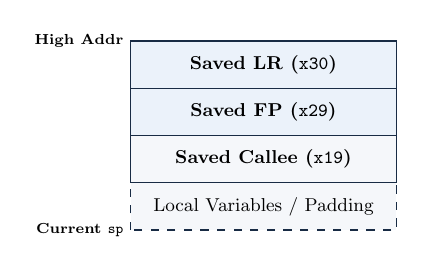
\begin{tikzpicture}[scale=0.75, every node/.style={transform shape}]
  \draw[fill=lightblue, draw=navy] (0,3.6) rectangle (4.5,4.4) node[midway, font=\small\bfseries] {Saved LR (\bits{x30})};
  \draw[fill=lightblue, draw=navy] (0,2.8) rectangle (4.5,3.6) node[midway, font=\small\bfseries] {Saved FP (\bits{x29})};
  \draw[fill=softgray, draw=navy] (0,2.0) rectangle (4.5,2.8) node[midway, font=\small\bfseries] {Saved Callee (\bits{x19})};
  \draw[fill=softgray, draw=navy, dashed] (0,1.2) rectangle (4.5,2.0) node[midway, font=\small] {Local Variables / Padding};
  \node[anchor=east, font=\scriptsize\bfseries] at (0,4.4) {High Addr};
  \node[anchor=east, font=\scriptsize\bfseries] at (0,1.2) {Current \bits{sp}};
\end{tikzpicture}
\end{column}
\end{columns}
\end{frame}

\begin{frame}{Frame Pointer (\texttt{x29}) and Frame Records}

\begin{itemize}\setlength{\itemsep}{5pt}
  \item The \key{Frame Pointer (\bits{x29} / \bits{fp})} can provide a fixed reference point within the activation frame for accessing arguments and local variables.
  \item \key{Frame Pointer Conventions:}
  \begin{itemize}\setlength{\itemsep}{2pt}
    \item Under standard AAPCS64 profiles, functions may maintain a frame record linking saved \bits{x29} and \bits{x30}.
    \item When used, this creates a traceable chain of stack frames to assist debuggers (e.g., GDB) with backtraces.
    \item However, platform rules or optimization levels may permit omitting frame records or repurposing \bits{x29}.
  \end{itemize}
\end{itemize}

\vspace{0.4cm}
\centering
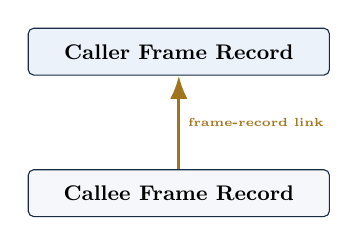
\begin{tikzpicture}[scale=0.85, every node/.style={transform shape}]
  \node[draw=navy, fill=lightblue, rounded corners=2pt, minimum width=4.5cm, minimum height=0.7cm, font=\small\bfseries] (caller) {Caller Frame Record};
  \node[draw=navy, fill=softgray, rounded corners=2pt, minimum width=4.5cm, minimum height=0.7cm, font=\small\bfseries, below=1.4cm of caller] (callee) {Callee Frame Record};
  \draw[-{Latex}, line width=1.2pt, gold!80!black] (callee.north) -- (caller.south) node[midway, right, font=\tiny\bfseries] {frame-record link};
\end{tikzpicture}
\end{frame}

% ============================================================
% Slide 19
% ============================================================

\begin{frame}[fragile]{Function Prologue Mechanics}
\begin{itemize}\setlength{\itemsep}{4pt}
  \item A \key{prologue} commonly allocates stack space and saves state needed by the function.
\end{itemize}
\vspace{0.05cm}
\begin{block}{Example Prologue Template}
\small
\begin{verbatim}
my_func:
    // Allocate 32 bytes and save FP/LR
    stp    x29, x30, [sp, #-32]!

    // x29 points to the frame record
    mov    x29, sp

    // Save callee-saved register used by the body
    str    x19, [sp, #16]
\end{verbatim}
\end{block}
\vspace{0.1cm}
\small
Pre-indexed \code{stp} combines stack-pointer writeback with the paired store of \bits{x29}/\bits{x30}.
\end{frame}

% ============================================================
% Slide 20
% ============================================================

\begin{frame}[fragile]{Function Epilogue Mechanics}

\begin{itemize}\setlength{\itemsep}{5pt}
  \item The \key{Epilogue} tears down the frame and restores state before returning.
  \item Reverses the exact sequence performed by the prologue:
\end{itemize}

\vspace{0.15cm}
\begin{block}{Standard Epilogue Template}
\small
\begin{verbatim}
    // 1. Restore saved callee registers
    ldr    x19, [sp, #16]

    // 2. Restore original FP and LR; release stack frame
    ldp    x29, x30, [sp], #32

    // 3. Return to caller
    ret
\end{verbatim}
\end{block}

\vspace{0.2cm}
\normalsize
Post-indexed \code{ldp} performs a paired architectural load and writeback in one instruction to restore \bits{x29}/\bits{x30} and deallocate 32 stack bytes.
\end{frame}

% ============================================================
% Slide 21
% ============================================================

\begin{frame}[fragile]{Local Variable Allocation on the Stack}
\begin{columns}[T,onlytextwidth]
\begin{column}{0.46\textwidth}
\begin{block}{C Function with Local Array}
\small
\begin{verbatim}
void process(void) {
    uint64_t buffer[2];
    buffer[0] = 10;
    buffer[1] = 20;
}
\end{verbatim}
\end{block}
\end{column}
\begin{column}{0.50\textwidth}
\begin{block}{Illustrative Leaf Stack Allocation}
\small
\begin{verbatim}
process:
    sub  sp, sp, #16

    mov  x0, #10
    str  x0, [sp, #0]
    mov  x0, #20
    str  x0, [sp, #8]

    add  sp, sp, #16
    ret
\end{verbatim}
\end{block}
\end{column}
\end{columns}
\vspace{0.2cm}
\small
Because this example is a leaf function, it does not need to save \bits{x30} solely for return linkage. The 16-byte local allocation preserves stack alignment.
\end{frame}

% ============================================================
% Slide 22
% ============================================================

\begin{frame}{Stack Alignment and Padding Rules}
\begin{itemize}\setlength{\itemsep}{4pt}
  \item AAPCS64 requires \bits{sp} to satisfy 16-byte alignment at public interfaces and when used for stack memory accesses.
  \item Frame allocation therefore rounds the required stack space up to a multiple of 16 bytes.
\end{itemize}
\vspace{0.1cm}
\begin{block}{Calculating Frame Size}
\[
\text{Frame Size} = \text{align}_{16}(\text{saved state} + \text{local storage})
\]
\end{block}
\vspace{0.1cm}
\begin{center}
\footnotesize
\renewcommand{\arraystretch}{1.12}
\begin{tabular}{>{\raggedright\arraybackslash}p{0.31\textwidth} >{\raggedright\arraybackslash}p{0.22\textwidth} >{\raggedright\arraybackslash}p{0.34\textwidth}}
\toprule
\textbf{Required Space} & \textbf{Frame Size} & \textbf{Example Allocation} \\
\midrule
16B saved FP/LR & 16 bytes & \code{stp x29, x30, [sp, \#-16]!} \\
16B saved FP/LR + 20B locals & 48 bytes & allocate a 48-byte frame and place saved state/locals within it \\
16B saved FP/LR + 32B locals & 48 bytes & allocate a 48-byte frame \\
\bottomrule
\end{tabular}
\end{center}
\end{frame}

% ============================================================
% Section 4 Divider
% ============================================================

\sectiondivider{PART 4}{Worked Assembly Examples \& Patterns}

% ============================================================
% Slide 23
% ============================================================

\begin{frame}[fragile]{Worked Example 1: Minimal Leaf Function}
\begin{block}{C Code: \texttt{int64\_t add\_three(int64\_t a, int64\_t b, int64\_t c)}}
\end{block}
\vspace{0.05cm}
\begin{block}{AArch64 Assembly Implementation}
\small
\begin{tabular}{lll}
\multicolumn{3}{l}{\textit{// Inputs: x0 = a, x1 = b, x2 = c}} \\
\code{add\_three:} & & \\
    & \code{add x0, x0, x1} & \text{\scriptsize // x0 = a + b} \\
    & \code{add x0, x0, x2} & \text{\scriptsize // x0 = (a + b) + c} \\
    & \code{ret}             & \text{\scriptsize // result already in x0} \\
\end{tabular}
\end{block}
\vspace{0.15cm}
\begin{itemize}\setlength{\itemsep}{2pt}
  \item Calls no subroutines and needs no stack allocation.
  \item The function consists of three architectural instructions.
\end{itemize}
\end{frame}

% ============================================================
% Slide 24
% ============================================================

\begin{frame}[fragile]{Worked Example 2: Non-Leaf Nested Function}
\begin{block}{C Code: \texttt{int64\_t compute(int64\_t x)}}
\small
\code{return add\_three(x, 10, 20);}
\end{block}
\vspace{0.05cm}
\begin{block}{AArch64 Assembly Implementation}
\footnotesize
\begin{tabular}{lll}
\multicolumn{3}{l}{\textit{// Input: x0 = x}} \\
\code{compute:} & & \\
 & \code{stp x29, x30, [sp, \#-16]!} & \text{\scriptsize // save FP and LR} \\
 & \code{mov x29, sp}                  & \text{\scriptsize // establish frame record} \\
 & \code{mov x1, \#10}                 & \text{\scriptsize // 2nd argument} \\
 & \code{mov x2, \#20}                 & \text{\scriptsize // 3rd argument} \\
 & \code{bl  add\_three}               & \text{\scriptsize // nested call overwrites x30} \\
 & \code{ldp x29, x30, [sp], \#16}     & \text{\scriptsize // restore FP/LR} \\
 & \code{ret}                           & \text{\scriptsize // return to caller} \\
\end{tabular}
\end{block}
\end{frame}

% ============================================================
% Slide 25
% ============================================================

\begin{frame}[fragile]{Worked Example 3: Recursive Factorial}
\begin{columns}[T,onlytextwidth]
\begin{column}{0.36\textwidth}
\begin{block}{C Logic}
\scriptsize
\begin{verbatim}
uint64_t factorial(uint64_t n) {
  if (n <= 1) return 1;
  return n * factorial(n - 1);
}
\end{verbatim}
\end{block}
\vspace{0.05cm}
\scriptsize
Each invocation preserves its own return address and the current value of \code{n} across the recursive call.
\end{column}
\begin{column}{0.60\textwidth}
\begin{block}{AArch64 Assembly}
\tiny
\begin{verbatim}
factorial:
    cmp  x0, #1
    b.ls .Lbase

    stp  x29, x30, [sp, #-32]!
    mov  x29, sp
    str  x19, [sp, #16]
    mov  x19, x0
    sub  x0, x0, #1
    bl   factorial
    mul  x0, x0, x19
    ldr  x19, [sp, #16]
    ldp  x29, x30, [sp], #32
    ret

.Lbase:
    mov  x0, #1
    ret
\end{verbatim}
\end{block}
\end{column}
\end{columns}
\end{frame}

% ============================================================
% Slide 26
% ============================================================

\begin{frame}[fragile]{Worked Example 4: Passing More Than 8 Arguments}
\begin{block}{Example Assumption}
This example uses ten 64-bit integer arguments. Arguments 1--8 use \bits{x0}--\bits{x7}; the remaining arguments are placed in the stack argument area.
\end{block}
\vspace{0.05cm}
\begin{columns}[T,onlytextwidth]
\begin{column}{0.48\textwidth}
\begin{block}{Caller Side}
\small
\begin{verbatim}
// Prepare 9th and 10th arguments
mov  x9,  #100
mov  x10, #200
stp  x9, x10, [sp, #-16]!

bl   func_with_10_args

add  sp, sp, #16
\end{verbatim}
\end{block}
\end{column}
\begin{column}{0.48\textwidth}
\begin{block}{Callee Side}
\small
\begin{verbatim}
func_with_10_args:
    // Args 1-8 are in x0-x7
    ldr  x9,  [sp, #0]   // 9th arg
    ldr  x10, [sp, #8]   // 10th arg
    ret
\end{verbatim}
\end{block}
\end{column}
\end{columns}
\end{frame}

% ============================================================
% Slide 27
% ============================================================

\begin{frame}{Common Function Linkage Bugs in Assembly}
\begin{itemize}\setlength{\itemsep}{5pt}
  \item \key{1. Overwriting the Return Address:} A nested \code{bl} overwrites \bits{x30}; failing to preserve the incoming return address can return control to the wrong location.
  \item \key{2. Corrupting Callee-Saved Registers:} Modifying \bits{x19}--\bits{x28} without restoring them violates the calling convention.
  \item \key{3. Stack Misalignment:} Violating AAPCS64 stack-alignment rules breaks ABI assumptions and can fault where SP-alignment checking is enabled.
  \item \key{4. Unbalanced Stack Pointer:} Failing to restore \bits{sp} correctly can corrupt stack-resident state and later restores.
\end{itemize}
\end{frame}

% ============================================================
% Section 5 Divider
% ============================================================

\sectiondivider{SUMMARY \& ASSESSMENT}{Review and Self-Test Questions}

% ============================================================
% Slide 28: Comprehensive Summary
% ============================================================

\begin{frame}{Topic 6: Comprehensive Summary}
\begin{itemize}\setlength{\itemsep}{5pt}
  \item \key{Linkage Primitives:} \code{bl}/\code{blr} write the return address to \bits{x30}; \code{ret} normally returns through \bits{x30}.
  \item \key{AAPCS64 Register Contract:}
  \begin{itemize}\setlength{\itemsep}{1.5pt}
    \item Scalar arguments commonly begin in \bits{x0}--\bits{x7}; most scalar results return in \bits{x0}.
    \item \bits{x0}--\bits{x17} are caller-saved; \bits{x19}--\bits{x28} are callee-saved.
  \end{itemize}
  \item \key{Activation Frames:} Stack frames hold saved linkage state, preserved registers, and local storage while maintaining required alignment.
  \item \key{Prologue/Epilogue:} Paired \code{stp}/\code{ldp} instructions commonly save and restore \bits{x29}/\bits{x30} while updating \bits{sp}.
\end{itemize}
\end{frame}

% ============================================================
% Slide 29: Self-Test Questions (Part 1)
% ============================================================

\begin{frame}{Self-Test Questions: Linkage \& AAPCS64}

\begin{enumerate}\setlength{\itemsep}{6pt}
  \item \key{Leaf vs.\ Non-Leaf Function Linkage:} How do leaf and non-leaf functions differ regarding link-register management and return-address preservation?

  \item \key{Register Preservation Contracts:} Suppose function \code{foo()} calls \code{bar()}. If \code{foo()} needs to maintain a loop counter value across the call, should it store that counter in \bits{x9} or \bits{x19}? Why?

  \item \key{Parameter Passing Limits:} How are integer parameters handled when calling a C function declared with 10 scalar arguments: \code{void test(int a1, ..., int a10)}?
\end{enumerate}

\end{frame}

% ============================================================
% Slide 30: Self-Test Questions (Part 2)
% ============================================================

\begin{frame}{Self-Test Questions: Stack Frame Management}

\begin{enumerate}\setlength{\itemsep}{6pt}
  \item \key{Stack Allocation Alignment:} A non-leaf function saves \bits{x29}/\bits{x30} (16 bytes) and needs 20 bytes of local buffer space. What is the minimum frame size it must allocate on the stack to maintain AAPCS64 compliance?

  \item \key{Prologue/Epilogue Verification:} Identify the bug in the following epilogue:
  \small
  \begin{tabular}{l}
  \code{ldp x29, x30, [sp], \#16} \\
  \code{ldr x19, [sp, \#16]} \\
  \code{ret} \\
  \end{tabular}

  \item \key{Frame Pointer Chains:} When frame records are maintained, how does saved \bits{x29} help a debugger reconstruct the call chain?
\end{enumerate}

\end{frame}


% ============================================================
% Looking Ahead
% ============================================================

\begin{frame}{Looking Ahead}
\begin{block}{Next Lecture Preview}
\key{Our Next Topic:}
Machine Code \& AArch64 Instruction Encoding
\end{block}
\vfill
\begin{itemize}\setlength{\itemsep}{7pt}
  \item \key{32-Bit Instruction Words:} Relating assembly syntax to fixed-width A64 machine instructions.
  \item \key{Encoding Fields:} Identifying opcode, register, immediate, and shift fields within instruction formats.
  \item \key{Assembly to Machine Code:} Building and interpreting representative AArch64 instruction encodings.
\end{itemize}
\vfill
\end{frame}

\end{document}